\documentclass{article}
\usepackage[utf8]{inputenc}

\usepackage{sectsty}
\usepackage{fancyhdr}
\usepackage[top=1.25cm, bottom=2cm, left=2cm, right=2cm]{geometry}
\usepackage{tabularx,tabulary}
\usepackage{graphicx}
\date{3 Avril 2019}
\author{FRANCESCHETTI Maël\\KADOCH Daoud\\MANSON Fabien\\CASTANET Nicolas}
\title{\LARGE{Projet 3i013\\}Rapport de Projet}

\usepackage[french]{babel}
%\usepackage[utf8x]{inputenc}
%\usepackage{amsmath}
%\usepackage[colorinlistoftodos]{todonotes}
\begin{document}

\begin{titlepage}

\newcommand{\HRule}{\rule{\linewidth}{0.5mm}} % Defines a new command for the horizontal lines, change thickness here

\center % Center everything on the page
 
%----------------------------------------------------------------------------------------
%	HEADING SECTIONS
%----------------------------------------------------------------------------------------

\textsc{\LARGE Université Sorbonne}\\[3cm] % Name of your university/college
\textsc{\Large Licence Informatique 3\up{ème} Année}\\[0.5cm] % Major heading such as course name
\textsc{\large Projet 3i013}\\[2cm] % Minor heading such as course title

%----------------------------------------------------------------------------------------
%	TITLE SECTION
%----------------------------------------------------------------------------------------

\HRule \\[0.4cm]
{ \huge \bfseries Rapport de Projet}\\[0.4cm] % Title of your document
\HRule \\[2cm]
 
%----------------------------------------------------------------------------------------
%	AUTHOR SECTION
%----------------------------------------------------------------------------------------

\begin{minipage}{0.4\textwidth}
	\begin{flushleft} \large
	\emph{Auteurs:}\\[0.2cm]
	Nicolas \textsc{CASTANET}\\ % Your name
	Maël \textsc{FRANCESCHETTI}\\ % Your name
	Daoud \textsc{KADOCH}\\ % Your name
	Fabien \textsc{MANSON} % Your name
	\end{flushleft}
\end{minipage}
~
\begin{minipage}{0.4\textwidth}
	\begin{flushright} \large
	\emph{Enseignant:} \\[0.2cm]
	Fabrice \textsc{KORDON}
	\end{flushright}
\end{minipage}\\[4cm]

%----------------------------------------------------------------------------------------
%	DATE SECTION
%----------------------------------------------------------------------------------------

{\large 2 Avril 2019}\\[3cm] % Date, change the \today to a set date if you want to be precise

%----------------------------------------------------------------------------------------
%	LOGO SECTION
%----------------------------------------------------------------------------------------


\includegraphics[scale=0.15]{logo_sorbonne.png} % Include a department/university logo - this will require the graphicx package
 
%----------------------------------------------------------------------------------------

\vfill % Fill the rest of the page with whitespace

\end{titlepage}

% -----------------------------------------------------
\newpage
\renewcommand{\contentsname}{\center{Table des Matières}\vspace*{5cm}}

\tableofcontents



\newpage
\section{Présentation du Projet}
	\subsection{Contexte}
		Un client souhaite effectuer un vol autonome avec un drone Bebop 2 tout en visualisant sur un iPod Touch le retour vidéo de la caméra embarquée sur le drone. L'iPod sera placé dans un masque de vue à la première personne. \\	
		%Le client souhaite faire effectuer des vols autonomes à un drone Bebop 2, avec un retour vidéo en temps réel sur un iPod Touch. Ce dernier pourra être placé dans un masque de vue à la première personne.\\
		La solution devra permettre à l'utilisateur de saisir un plan de vol sur une carte interactive et de le faire exécuter par le drone tout en ayant un retour vidéo sur l'iPod.\\
		

	\subsection{Use Case}	
	    \subsubsection{Création d'un plan de vol}
	    Dans le premier cas d'utilisation, l'utilisateur souhaite créer un nouveau plan de vol afin de le faire suivre à son drone dans le futur, voici les étapes qu'il va suivre:
	    
	    \vspace{0.7cm}	     
	    \begin{center}
	    \renewcommand{\arraystretch}{2}
        \begin{tabularx}{15cm}{|c|X|}
            \hline
            1 & L'utilisateur lance l'application et arrive sur la page d'accueil.\\
            \hline
            2 & L'utilisateur lance la fonctionnalité de saisie du plan de vol sur une machine connectée au réseau local.\\
            \hline
            3 & L'utilisateur saisit le plan de vol sur la carte en spécifiant les points de passage du drone ainsi que les altitudes que le drone doit adopter au cours du vol. \\
            \hline
            4 & L'utilisateur valide la saisie de son plan de vol, ce dernier est enregistré. \\
            \hline
        \end{tabularx}
        \end{center}
        
	    \vspace{0.8cm}
	    
	    \subsubsection{Exécution d'un plan de vol}
	    Dans le deuxième cas d’utilisation, l'utilisateur possède déjà un ou plusieurs plan de vol enregistrés sur sa machine, par exemple le tour de son énorme jardin qu'il souhaite surveiller sans avoir à ce déplacer. Il fais désormais exécuter au drone l'un de ces plan de vol et observe le retour vidéo sur son Ipod.
	    Voici les étapes suivient :
	    
	    \vspace{0.7cm}	     
	    \begin{center}
	    \renewcommand{\arraystretch}{2}
        \begin{tabularx}{15cm}{|c|X|}
            \hline
            1 & L'utilisateur lance l'application et arrive sur la page d'accueil.\\
            \hline
            5 & L'utilisateur allume le drone et y connecte sa machine en wifi. \\
            \hline
            6 & L'utilisateur lance la fonctionnalité d'exécution du plan de vol. \\
            \hline
            7 &  L'utilisateur démarre l'iPod touch, le connecte au réseau local et lance l'application de réception vidéo. La réception vidéo en temps réel sur l'iPod commence.\\
            \hline
            8 & L'utilisateur sélectionne parmi les plans de vols présents sur le drone celui qu'il souhaite réaliser. \\
            \hline
            9 & L'utilisateur place l'iPod dans le masque FPV, l'enfile, puis lance l'exécution du plan de vol d'un mouvement de tête. Le drone décolle. \\
            \hline
            10 & Le drone effectue le plan de vol choisi, l'utilisateur voit en temps réel ce que le drone filme et peut constater l'état d'enneigement de son jardin. \\
            \hline
            11 & L'utilisateur attend la fin de l'exécution du plan de vol pour retirer le masque et aller récupérer le drone une fois qu'il aura atterri à son point de départ, comme prévu.\\
            \hline 
\end{tabularx}
        \end{center}
	    



% CAHIER DES CHARGES %

\newpage
\subsection{Cahier des charges}
\subsubsection{Présentation du Projet}
	\subsubsubsection{Contexte et définition du problème}
		Un client nous contacte dans le but de réaliser une application lui permettant d'effectuer un vol autonome avec un drone Bebop 2 tout en visualisant sur un iPod Touch le retour vidéo de la caméra embarquée sur le drone. L'iPod sera placé dans un masque de vue à la première personne. \\	
		%Le client souhaite faire effectuer des vols autonomes à un drone Bebop 2, avec un retour vidéo en temps réel sur un iPod Touch. Ce dernier pourra être placé dans un masque de vue à la première personne.\\
		La solution devra permettre à l'utilisateur de saisir un plan de vol sur une carte interactive et de le faire exécuter par le drone tout en ayant un retour vidéo sur l'iPod.\\
		\medbreak
        \begin{flushleft}
	    \textbf{Cas d'utilisation :} \\
	    \end{flushleft}
	    1) Un utilisateur souhaite effectuer une ronde avec un drone pour surveiller sa propriété (qui possède un très grand jardin) au prix d'un moindre effort.\\
	    Voici un exemple des étapes qu'il va suivre chronologiquement :\\
		[1cm]	     
	    \begin{center}
	    \renewcommand{\arraystretch}{2}
        \begin{tabularx}{15cm}{|c|X|}
            \hline
            1 & L'utilisateur lance l'application et arrive sur la page d'accueil.\\
            \hline
            2 & L'utilisateur lance la fonctionnalité de saisie du plan de vol sur une machine connectée au réseau local.\\
            \hline
            3 & L'utilisateur saisit le plan de vol sur la carte en spécifiant les points de passage du drone ainsi que les altitudes que le drone doit adopter au cours du vol. \\
            \hline
            4 & L'utilisateur valide la saisie de son plan de vol, ce dernier est enregistré. \\
            \hline
            5 & L'utilisateur allume le drone et y connecte sa machine en wifi. \\
            \hline
            6 & L'utilisateur lance la fonctionnalité d'exécution du plan de vol. \\
            \hline
            7 &  L'utilisateur démarre l'iPod touch, le connecte au réseau local et lance l'application de réception vidéo. La réception vidéo en temps réel sur l'iPod commence.\\
            \hline
            8 & L'utilisateur sélectionne parmi les plans de vols présents sur le drone celui qu'il vient de réaliser. \\
            \hline
            9 & L'utilisateur place l'iPod dans le masque FPV, le met sur sa tête, puis lance l'exécution du plan de vol. Le drone décolle. \\
            \hline
            10 & Le drone effectue le plan de vol choisi, l'utilisateur voit en temps réel ce que le drone filme. \\
            \hline
            11 & L'utilisateur souhaite stopper l'exécution de plan de vol : par exemple, il a repéré quelque chose d'anormal sur la zone de vol et souhaite s'y rendre au plus vite. Il active alors la procédure d'arrêt d'urgence sur sa machine et retire le masque FPV. Le drone stoppe l'exécution du plan de vol et attérit sur place si les conditions le permettent. \\
            \hline
        \end{tabularx}
        \end{center}
        
        \newpage
        2) En hiver, un utilisateur souhaite faire effectuer au drone le tour de son jardin pour contrôler le niveau d'enneigement de celui-ci sans risquer de glisser.\\
        Voici un exemple des étapes qu'il va suivre chronologiquement : \\ [1cm]
	    \begin{center}
	    \renewcommand{\arraystretch}{2}
        \begin{tabularx}{15cm}{|c|X|}
            \hline
            1 & L'utilisateur lance l'application et arrive sur la page d'accueil.\\
            \hline
            2 & L'utilisateur lance la fonctionnalité de saisie du plan de vol sur une machine connectée au réseau local.\\
            \hline
            3 & L'utilisateur saisit le plan de vol sur la carte en spécifiant les points de passage du drone tout autour de son jardin et spécifie une altitude de quelques mètres. Le tracé est fait de manière à faire revenir le drone à son point de départ après avoir fait le tour du jardin. \\
            \hline
            4 & L'utilisateur valide la saisie de son plan de vol, ce dernier est enregistré. \\
            \hline
            5 & L'utilisateur allume le drone et y connecte sa machine en wifi. \\
            \hline
            6 & L'utilisateur lance la fonctionnalité d'exécution du plan de vol. \\
            \hline
            7 &  L'utilisateur démarre l'iPod touch, le connecte au réseau local et lance l'application de réception vidéo. La réception vidéo en temps réel sur l'iPod commence.\\
            \hline
            8 & L'utilisateur sélectionne parmi les plans de vols présents sur le drone celui qu'il vient de réaliser. \\
            \hline
            9 & L'utilisateur place l'iPod dans le masque FPV, le met sur sa tête, puis lance l'exécution du plan de vol. Le drone décolle. \\
            \hline
            10 & Le drone effectue le plan de vol choisi, l'utilisateur voit en temps réel ce que le drone filme et peut constater l'état d'enneigement de son jardin. \\
            \hline
            11 & L'utilisateur attend la fin de l'exécution du plan de vol pour retirer le masque et aller récupérer le drone une fois qu'il aura atterri à son point de départ, comme prévu.\\
            \hline 
        \end{tabularx}
        \end{center}
        \vspace*{1cm}
	\subsubsubsection{Objectifs}
		%\vspace*{0.3cm}
		\begin{enumerate}
        	\item Permettre à l'utilisateur de saisir un plan de vol étape par étape sur une carte interactive et de spécifier les altitudes du drone à chaque point de passage.
        	\item Permettre à l'utilisateur de sauvegarder son plan de vol pour le réutiliser plus tard.
			\item Permettre à l'utilisateur de lancer l'exécution du plan de vol réalisé au préalable.
		 	\item Rediriger le flux vidéo du drone vers l'iPod Touch. 
		 	\item Minimiser les latences vidéo (de l'ordre de la seconde).
		 	\item Permettre d'arrêter le vol en cours en cas d'urgence.
		\end{enumerate}
		
	\newpage
\subsubsection{Besoins fonctionnels}
    \subsubsubsection{Fonctionnalités requises}
	    \begin{center}
	    \vspace*{0.7cm}
        \begin{tabularx}{15cm}{|c|p{4cm}|X|}
            \hline
            1 & Saisie du plan de vol & L'utilisateur doit pouvoir saisir un plan de vol sur une carte à travers une interface intuitive. L'utilisateur doit pouvoir spécifier l'altitude du drone à chaque waypoint (point de passage).\\
            \hline
            2 & Traduction du plan de vol au format Mavlink & Le plan de vol saisi graphiquement par l'utilisateur doit être converti au format Mavlink pour être ensuite envoyé au drone.\\
            \hline
            3 & Envoi du plan de vol au drone & La solution doit prendre en charge la récupération du plan de vol réalisé au préalable et son envoi au drone. \\
            \hline
            4 & Choix du plan de vol  & L'utilisateur doit pouvoir choisir le plan de vol enregistré sur le drone qu'il souhaite exécuter. \\
            \hline
            5 & Exécution du plan de vol  & Une fois le plan de vol choisi, l'utilisateur doit pouvoir en lancer l'exécution. \\
            \hline
            6 & Retour vidéo  & Tout au long du vol du drone, le retour vidéo de ce dernier doit être envoyé sur un iPod touch en temps réel et avec une latence minimale. \\
            \hline
            7 & Arrêt d'urgence  & À tout moment un deuxième utilisateur doit pouvoir enclencher un arrêt d'urgence depuis le PC. \\
            \hline
            8 & Démarrage de la ronde à l'aide de gestes & L'utilisateur pourra éventuellement engager le démarrage du vol en effectuant un certain mouvement de la tête. 	\\
			\hline
			9 & Arrêt d'urgence & L'utilisateur pourra éventuellement engager un arrêt d'urgence en effectuant par exemple un certain mouvement de la tête. 	\\
			\hline
        \end{tabularx}
        \end{center}

	\subsubsubsubsection{Diagramme des fonctionnalités \\}
	
	    Voici le diagramme des fonctionnalités (Figure 1) composé de l'utilisateur, du PC et du drone. L'iPod est ici considéré comme une extension de l'utilisateur, étant placé dans un masque FPV. On considère ici que le PC est déjà connecté au drone en Wifi et que l'iPod et le PC sont connecté tous les deux à un même réseau local.\\
	    
		\begin{center}
		\begin{figure}[!h]
		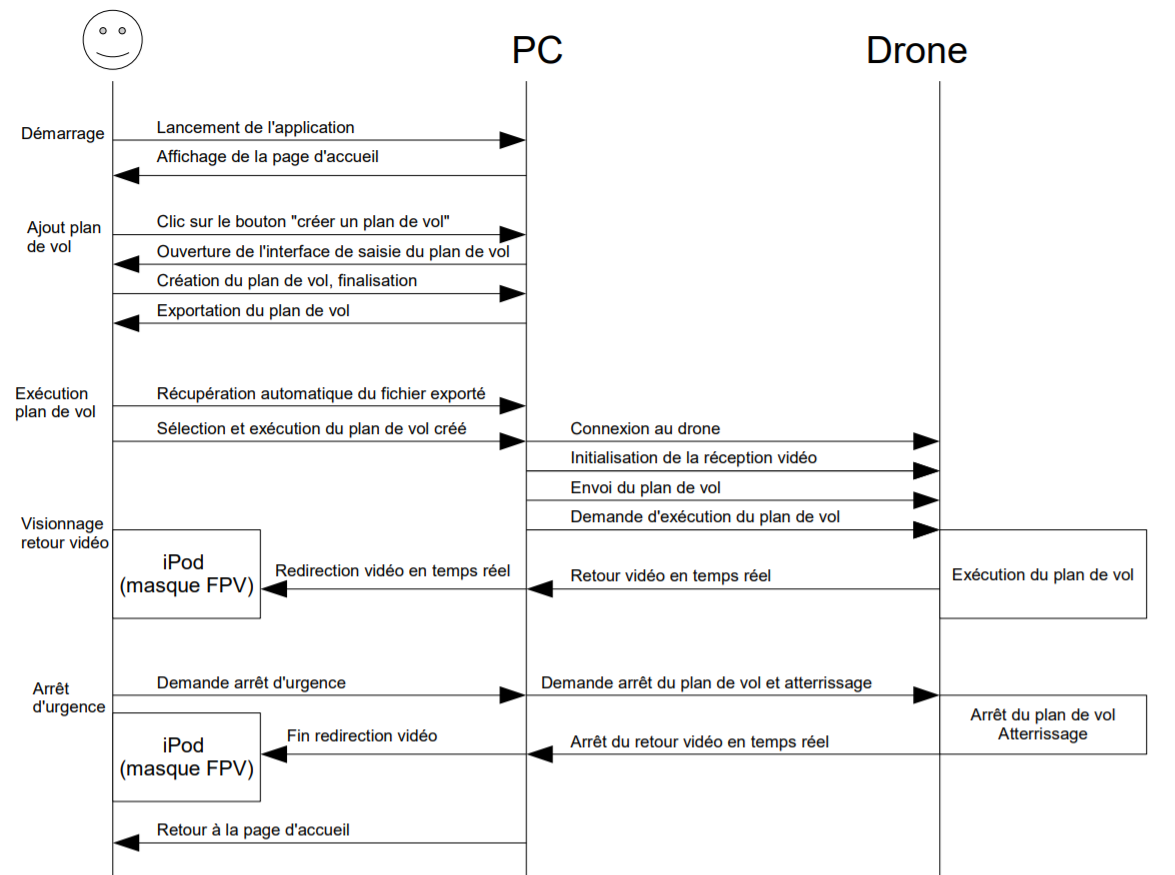
\includegraphics[scale=0.7]{corrige_diagramme_services.PNG}\\
		 \vspace*{0.3cm}
	%	Figure 1 - Diagramme des fonctionnalités
		\caption{Diagramme des fonctionnalités}
		\end{figure}
		\end{center}
		
		\newpage
			
\subsubsection{Périmètre}
	\subsubsubsection{À qui s'adresse le produit ?}
		Ce projet est destiné à un public désirant effectuer une ronde d'une durée de 20 à 25 minutes maximum avec son drone.\\
		La portée maximale du drone est de 200 mètres pour une altitude de 100 mètres tout au plus.
	
	\subsubsubsection{Les Limites}
		Le drone ne sera pas capable d'éviter les obstacles durant sa ronde, c'est à l'utilisateur d'établir un trajet cohérent avec son environnement.\\
		De plus, dans le cas où le trajet proposé est trop long par rapport à l'autonomie du drone, un simple message d'avertissement sera affiché pour prévenir l'utilisateur, l'application ne sera pas en mesure d'empêcher cette ronde.
	
	

	
\subsubsection{Ressources}
	\subsubsubsection{Matériel}

	    \textbf{Pour réaliser ce projet nous disposons du matériel suivant :}

		\begin{enumerate}
        \item Un drone Bebop 2.
        \item Un iPod Touch de 6ème génération sous iOS 12.
        \item Un accès aux salles machines SAR équipées de machines sous OSX.
        \item Un accès aux salles informatiques équipées de machines sous Linux.
        \end{enumerate}
        
	\subsubsubsection{L'équipe}

	L'équipe est composée de quatre étudiants en troisième année de licence d'informatique.\\
        Nos connaissances en programmation sous Linux sont bonnes mais le langage Objective-C et l'univers iOS nous sont pour le moment encore inconnus.

\subsubsection{Solutions étudiées}
	Au cours de nos recherches nous avons étudié principalement 3 solutions d'architecture envisageables pour le développement de l'application. Ces architectures sont les suivantes, de gauche à droite dans le tableau ci-après (figure 2): 
	  	\begin{enumerate}
        	\item Une architecture utilisant un PC sous linux pour la saisie du plan de vol et qui commande le drone, ainsi qu'un iPod Touch sur lequel on redirige le flux vidéo.
        	\item Une architecture utilisant un iPad pour la saisie du plan de vol, ainsi qu'un iPod Touch qui commande le drone et récupère le flux vidéo.
         	\item Une architecture utilisant un iPod Touch pour la saisie du plan de vol, qui commande le drone tout en récupérant le flux vidéo.\\
        \end{enumerate}
	\subsubsubsection{Comparatif des solutions}
	
		%________________		
		\begin{figure}[h]
		\begin{center}
		%\vspace*{0.7cm}
		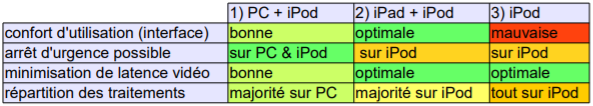
\includegraphics{comparatif_v3.PNG}\\
		\caption{tableau comparatif des solutions}
		\end{center}
		\end{figure}
		%________________
		

		%description précise du tableau        

		\indent Concernant le confort d'utilisation l'avantage est à la seconde solution car l'iPad possède un grand écran ainsi qu'une saisie tactile. La première solution est moins confortable principalement à cause de l'absence de saisie tactile sur le PC. La dernière solution n'est pas très pratique de fait de la petite taille de l'écran de l'iPod.\\
		
        \indent Concernant l'arrêt d'urgence c'est la première solution qui a l'avantage car elle permet d'implémenter cette fonction sur le PC ou sur l'iPod (via un mouvement de tête quand l'utilisateur porte le masque ou la pression d'une touche du clavier). L'arrêt d'urgence sur la troisième solution nous force à implémenter la fonctionnalité via un geste car l'iPod est, rappelons-le, attaché dans le masque donc difficile d'accès. La seconde solution ne pourra pas utiliser l'iPad pour lancer un arrêt d'urgence car l'iPod sera le seul appareil connecté au drone.\\
        
        \indent Les solutions 2 et 3 proposent une latence vidéo réduite car il n'y a pas à rediriger le flux vidéo. Ce dernier est directement reçu et lu par l'iPod. La première solution, en raison de la redirection du flux vidéo depuis le PC vers l'iPod, induit une latence légèrement plus importante (la différence reste assez imperceptible à l'utilisateur).\\
        
        \indent Et finalement en ce qui concerne les traitements réalisés par l'application, dans la première solution la majorité des calculs (saisie du plan de vol, envoie du plan de vol et traitement du flux vidéo reçu) seront fait sur le PC. L'iPod ne fera que recevoir le flux vidéo déjà traité. La seconde solution suit le même principe : la saisie du plan de vol se fait depuis l'iPad mais le traitement du flux vidéo ce fera sur l'iPod. Enfin la dernière solution traitera tout sur l'iPod ce qui peut causer des probleme d'autonomie de batterie pour l'iPod. L'avantage est donc à la première solution.\\ \\
        
        \indent Comme nous pouvons le constater, la solution utilisant le PC et l'iPod Touch est plus avantageuse dans la majorité des cas. C'est donc cette solution qui sera préférée.\\
        
        \indent Voici un schéma de l'architecture générale de la solution que nous avons choisie (figure 3).   
        %________________
 		\begin{figure}[!ht]
 		\begin{center}
 		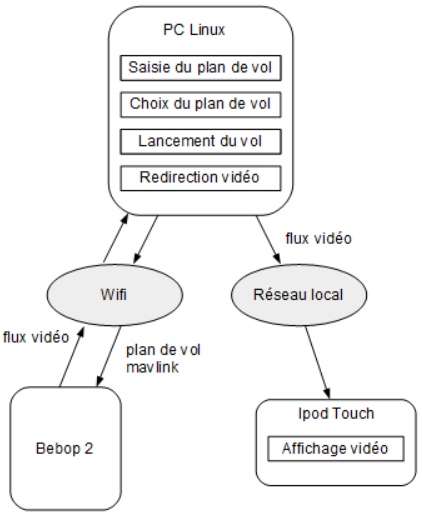
\includegraphics[scale=0.7]{Solution_PC.PNG}
 		\caption{Schéma de l'architecture générale de la solution retenue}
 		\end{center}
		\end{figure}
		%________________
\newpage
\subsubsection{Contraintes}

	\begin{flushleft}
	\textbf{Les contraintes techniques de la solution préférée sont :}
	\end{flushleft}
		\begin{enumerate}
        \item Le PC sous Linux doit avoir deux cartes réseau : une pour pouvoir se connecter au drone en wifi, l'autre pour se connecter au réseau local pour rediriger le flux vidéo.
        \item Il faut un réseau local sur lequel sont connectés le PC et l'iPod Touch.
        \item Le réseau local doit avoir un accès internet.
        \end{enumerate}
	
	\subsubsubsection{Délais}
		Le cahier des charges doit être envoyé au client pour le lundi 11 mars.\\
		En ce qui concerne le produit, il devra être prêt et livré début mai, et un rapport devra être rendu le jeudi 2 mai avant minuit.\\
		Une soutenance publique devant un jury se tiendra également début mai, nous viendrons y défendre l'ensemble de notre travail.\\
		
	\subsubsubsection{Autres contraintes}
	    \begin{flushleft}
	    \textbf{Concernant le plan de vol :} 
	    \end{flushleft}
	    	\begin{enumerate}
            	\item  L'application de saisie du plan de vol doit intégrer une carte interactive permettant de tracer ce dernier.
    		 	\item On devra pouvoir spécifier l'altitude à laquelle le drone doit se trouver aux différents points du parcours.
    		 	\item L'application devra au minimum pouvoir avertir l'utilisateur lorsqu'il tracera un trajet trop long pour le drone, tant pour son autonomie que pour la portée du signal wifi.
		 	\end{enumerate}
		
	    \begin{flushleft}
	    \textbf{Concernant le retour vidéo :}
	    \end{flushleft}
	     	\begin{enumerate}
	     	\item La qualité du retour vidéo est directement liée à la distance avec le serveur central (le PC) ainsi qu'à l'encombrement de l'espace dans lequel le drone vol. Un terrain avec des obstacles comme des bâtiments ou des arbres réduit fortement la porté du signal vidéo.
	     	\item Le retour vidéo du drone doit être envoyé à un iPod Touch en temps réel.
	     	\item Sa qualité doit être convenable (HD).
		 	\item La latence du retour vidéo sur l'iPod doit être minimale (de l'ordre de la seconde), et la vidéo doit être fluide.
		 	\end{enumerate}
\newpage
\subsubsection{Cinématique des écrans}
	
 	\begin{enumerate}
 	\item Lorsque l'utilisateur lance l'application, il arrive sur la page d'accueil (Figure 4). Il y a alors deux sections sur l'écran, l'une proposant d'ajouter un nouveau plan de vol et l'autre proposant d'exécuter un plan de vol parmi ceux existants.\\
 	Le bouton "créer un plan de vol" de la première section lance l'application de saisie du plan de vol. La sélection d'un plan de vol dans la seconde section et le clic sur le bouton "exécuter" lancent l'exécution par le drone du plan de vol choisi, le retour vidéo sur l'iPod peut alors commencer.\\
 	
 	 \begin{figure}[!h]
 	\begin{center}
 	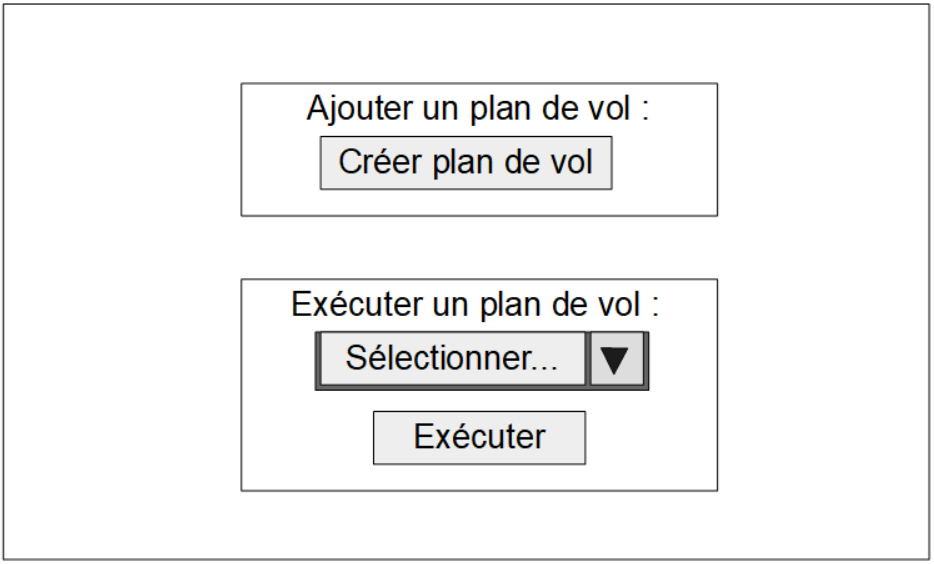
\includegraphics[scale=0.65]{maquette_appli_PC.PNG}
 	\caption{page d'accueil de l'application PC}
 	\end{center}
	\end{figure}
 	
 	\item Lors de l'ouverture de la page, la carte est vierge comme le montre la figure 5:\\
 	%________________
 	\begin{figure}[!h]
 	\begin{center}
 	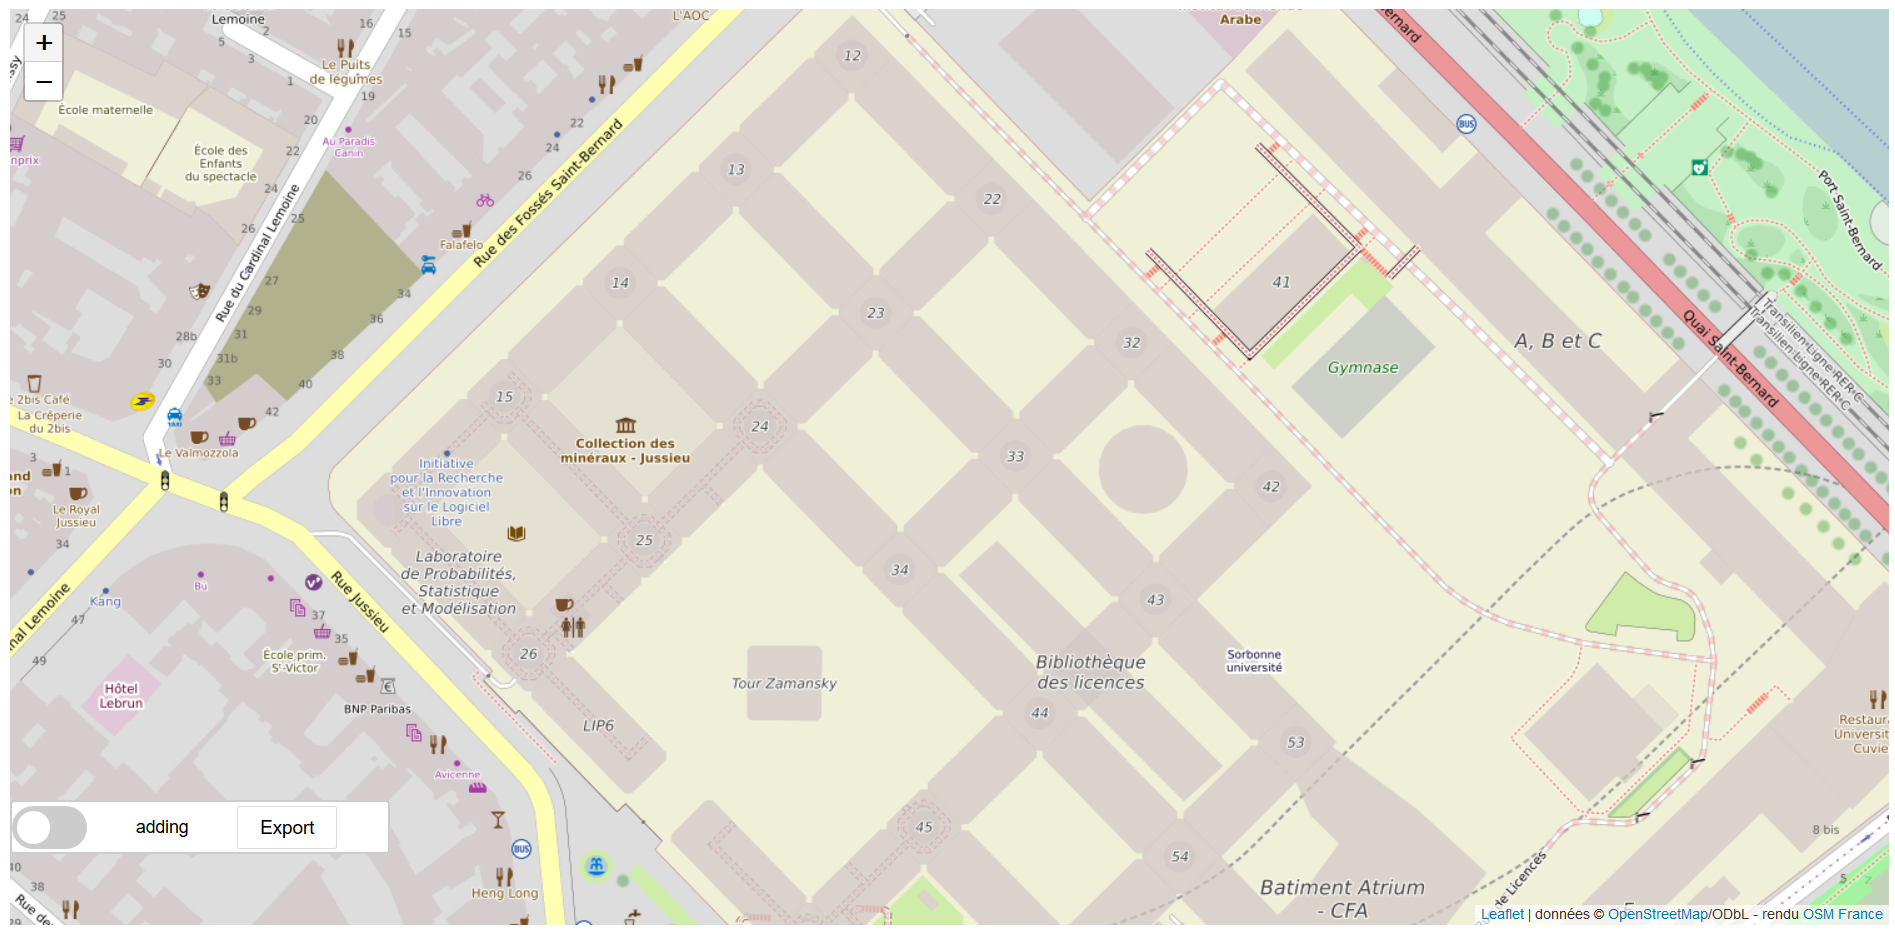
\includegraphics[scale=0.42]{capt1.PNG}
 	\caption{carte vierge}
 	\end{center}
	\end{figure}
	%________________
 	%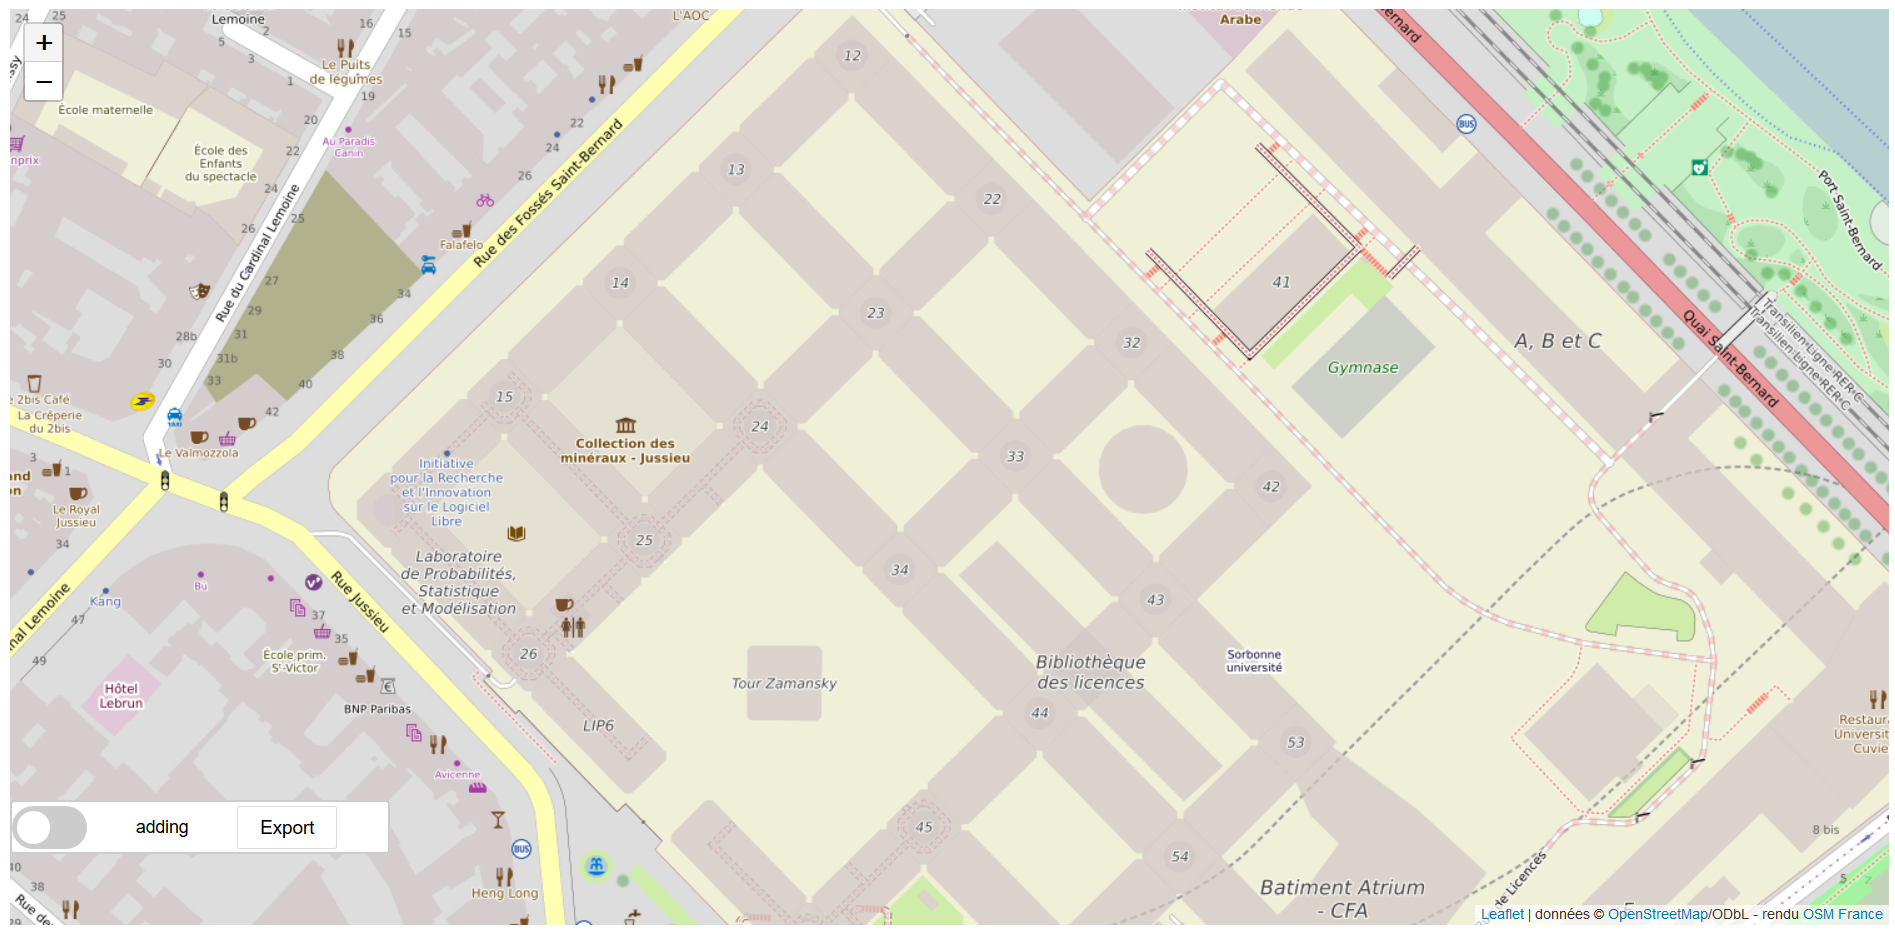
\includegraphics[scale=0.42]{capt1.PNG}\\
 	
 	La carte est interactive et on peut la déplacer avec la souris.
  Les boutons situés en haut à gauche permettent de zoomer et dézoomer sur la carte.\\ \\
 Le cadre situé en bas à gauche contient un switch (interrupteur) et un bouton : le switch permet de changer le mode d'interaction, et le bouton permet de finaliser le plan de vol en l'exportant dans un fichier.
 Il existe deux modes d'interraction :  le mode d'ajout et le mode de suppression. Le mode dans lequel on se situe est indiqué à coté du switch ("adding" / "removing").\\ \\
  En cliquant sur la carte, un marqueur est placé à l'endroit du clic. Chaque marqueur représente un point de passage du drone dans son itinéraire de vol. Les marqueurs peuvent être déplacés à la souris (drag and drop). Lors du survol de la souris sur un marqueur, une bulle indique son numéro d'ordre (0 pour le point de départ).\\
  	\begin{itemize}
 	\item En mode d'ajout, en cliquant sur un marqueur, on peut spécifier dans une boite de dialogue l'altitude à laquelle doit se situer le drone à ce point lors du vol.\\

 	\item En mode de suppression, en cliquant sur un marqueur, on supprime ce dernier. Les marqueurs sont alors automatiquement remis dans le bon ordre et le trajet est retracé.\\
	\end{itemize}
    \medbreak
   	%\newpage
   	%\vspace*{1cm}
   	\item On place des marqueurs en cliquant aux endroits voulus sur la carte. Au survol d'un marqueur, la bulle comportant son numéro d'ordre apparait :\\
 	%________________
 	\begin{figure}[!h]
 	\begin{center}
 	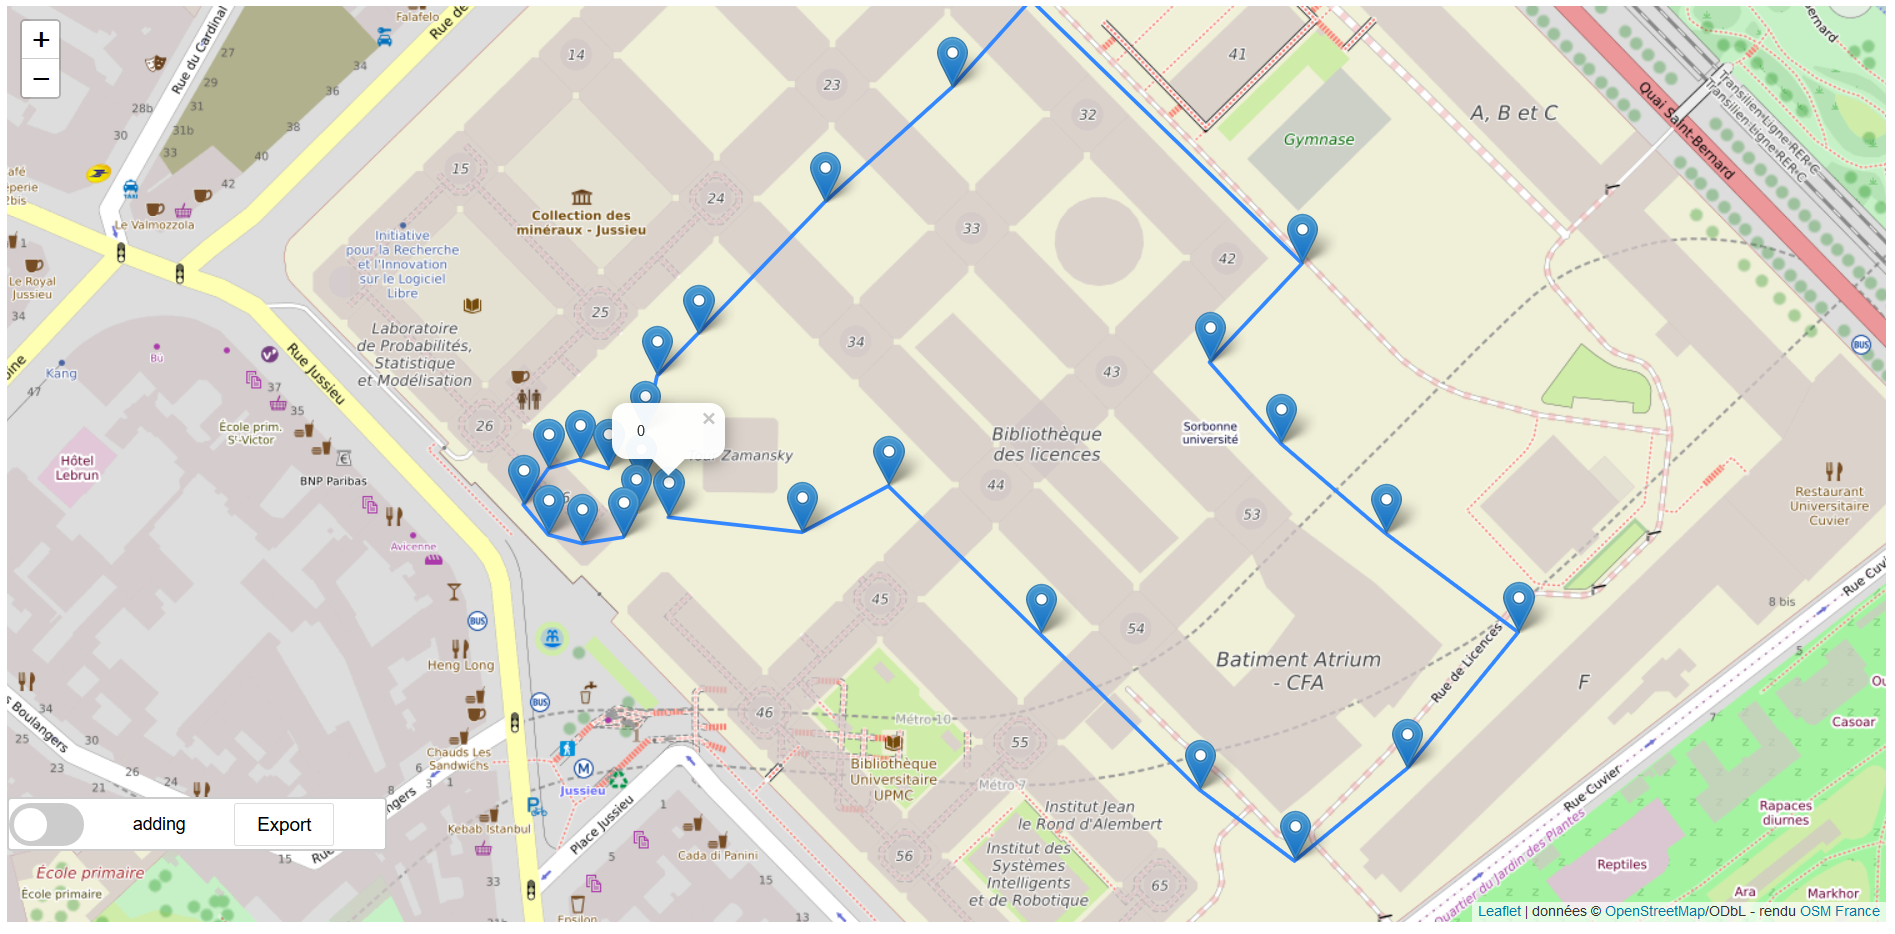
\includegraphics[scale=0.42]{capt3.PNG}
 	\caption{ajout de points de passage}
 	\end{center}
 	\end{figure}
 	%________________
 	%\vspace*{1.5cm}
 	\newpage
  	\item On souhaite retirer des marqueurs, on active le mode de suppression en cliquant sur le switch en bas à gauche (figure 7) et on clique ensuite sur les marqueurs à supprimer. L'ordre des marqueurs et le tracé du trajet s'adaptent :\\
	%________________	
	\begin{figure}[!h]
 	\begin{center}
 	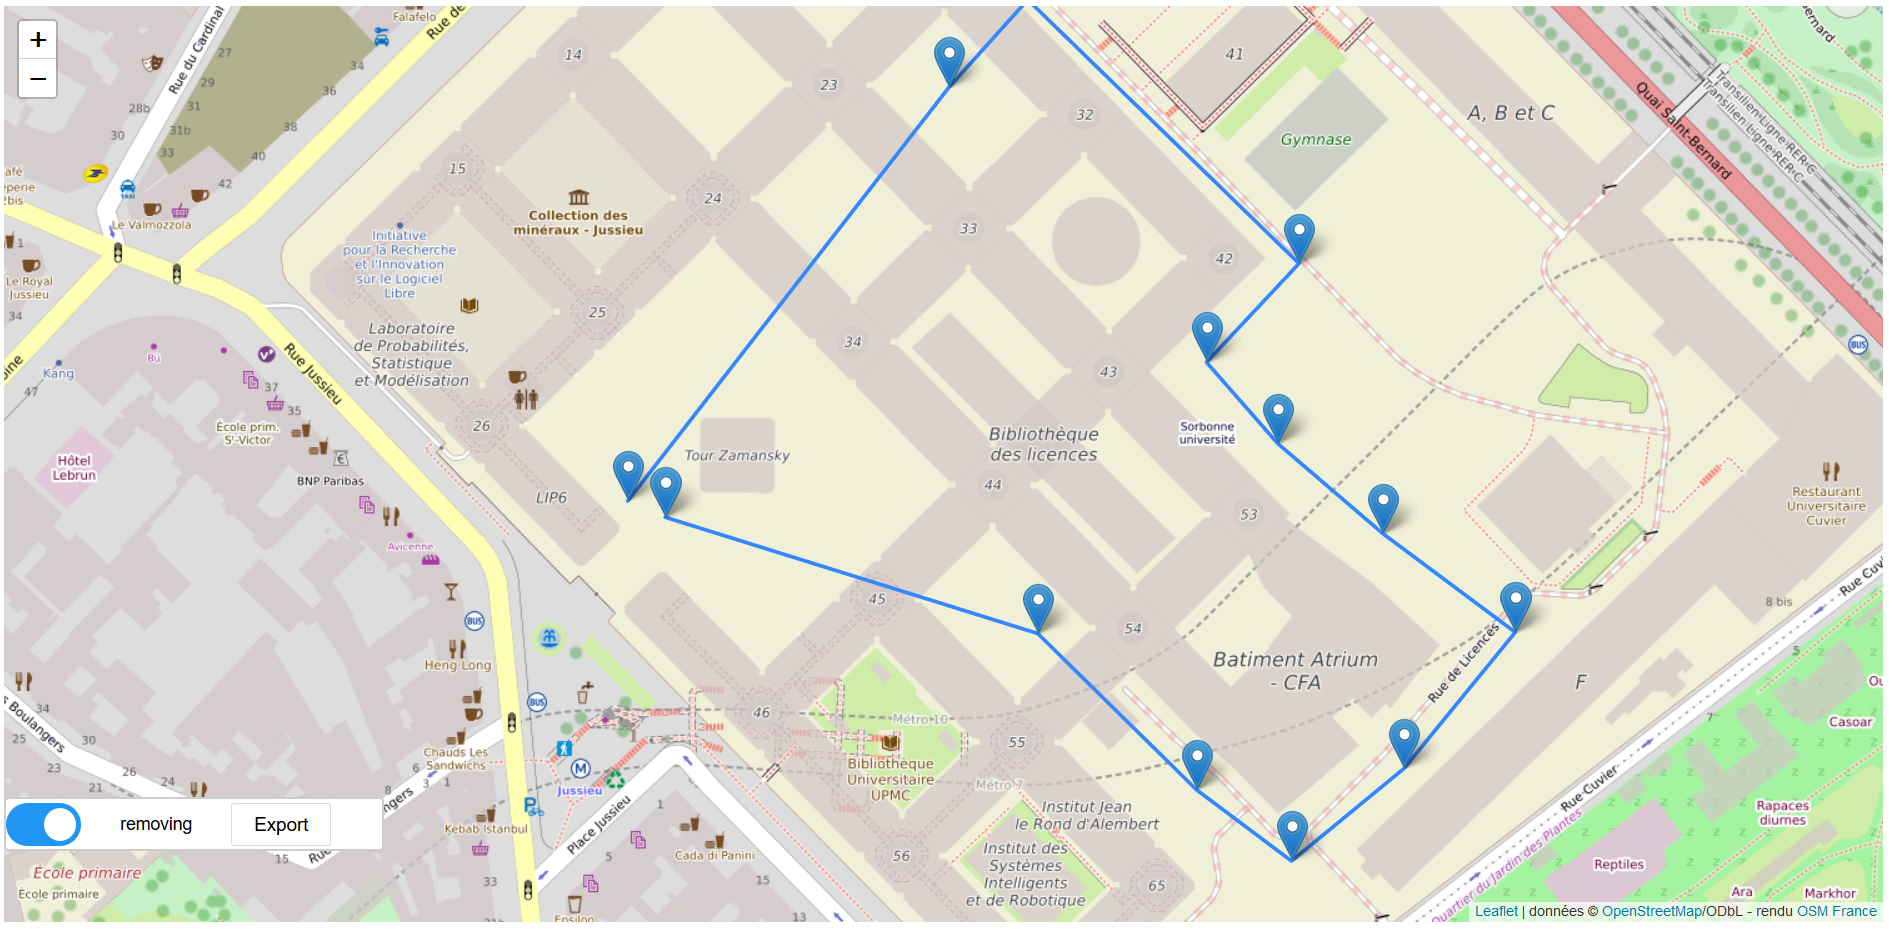
\includegraphics[scale=0.42]{capt5.PNG}
 	\caption{suppression de points de passage}
 	\end{center}
 	\end{figure}
 	%________________
	%\vspace*{0.5cm}

	\item On clique sur un marqueur pour spécifier l'altitude voulue à ce point (figure 8):\\
	%\vspace*{1cm}
	%________________
	\begin{figure}[!h]
 	\begin{center}
 	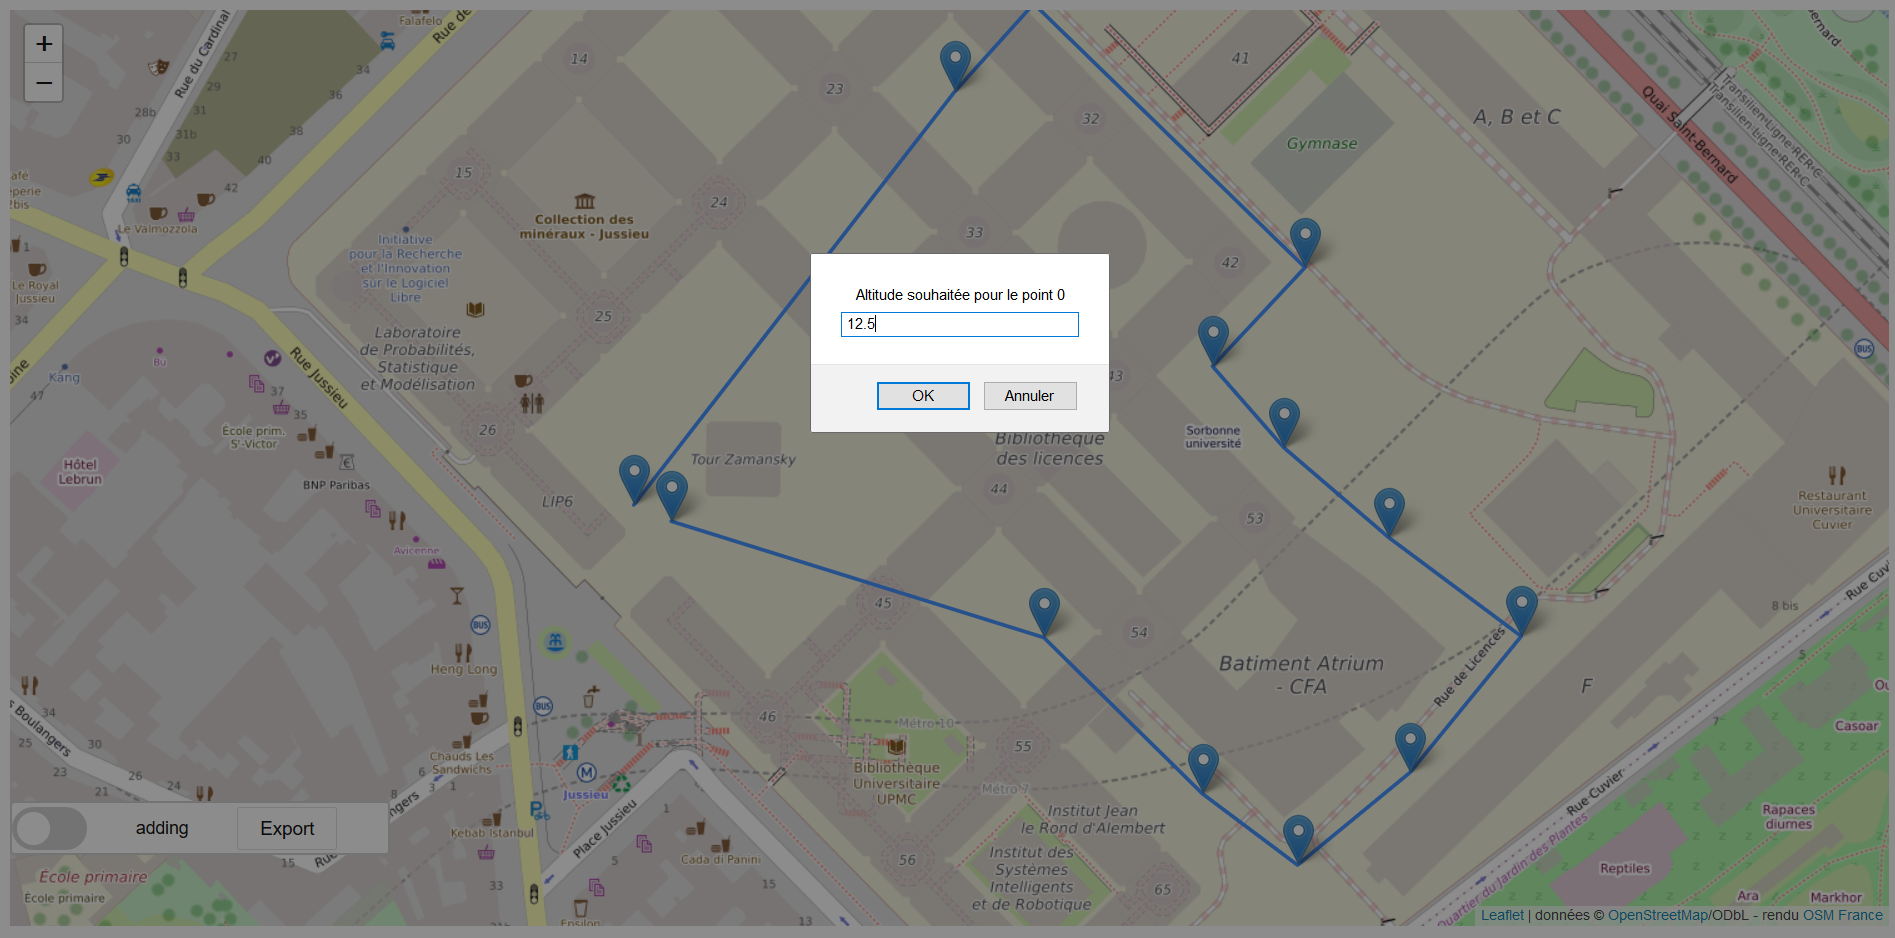
\includegraphics[scale=0.42]{capt6.PNG}
 	\caption{modification de l'altitude}
 	\end{center}
 	\end{figure}
 	%________________
 	\newpage 
 	
 	\item On peut déplacer les marqueurs avec un cliquer-glisser (drag and drop) sur ces derniers (figure 9):\\
 	%________________
 	\begin{figure}[!h]
 	\begin{center}
 	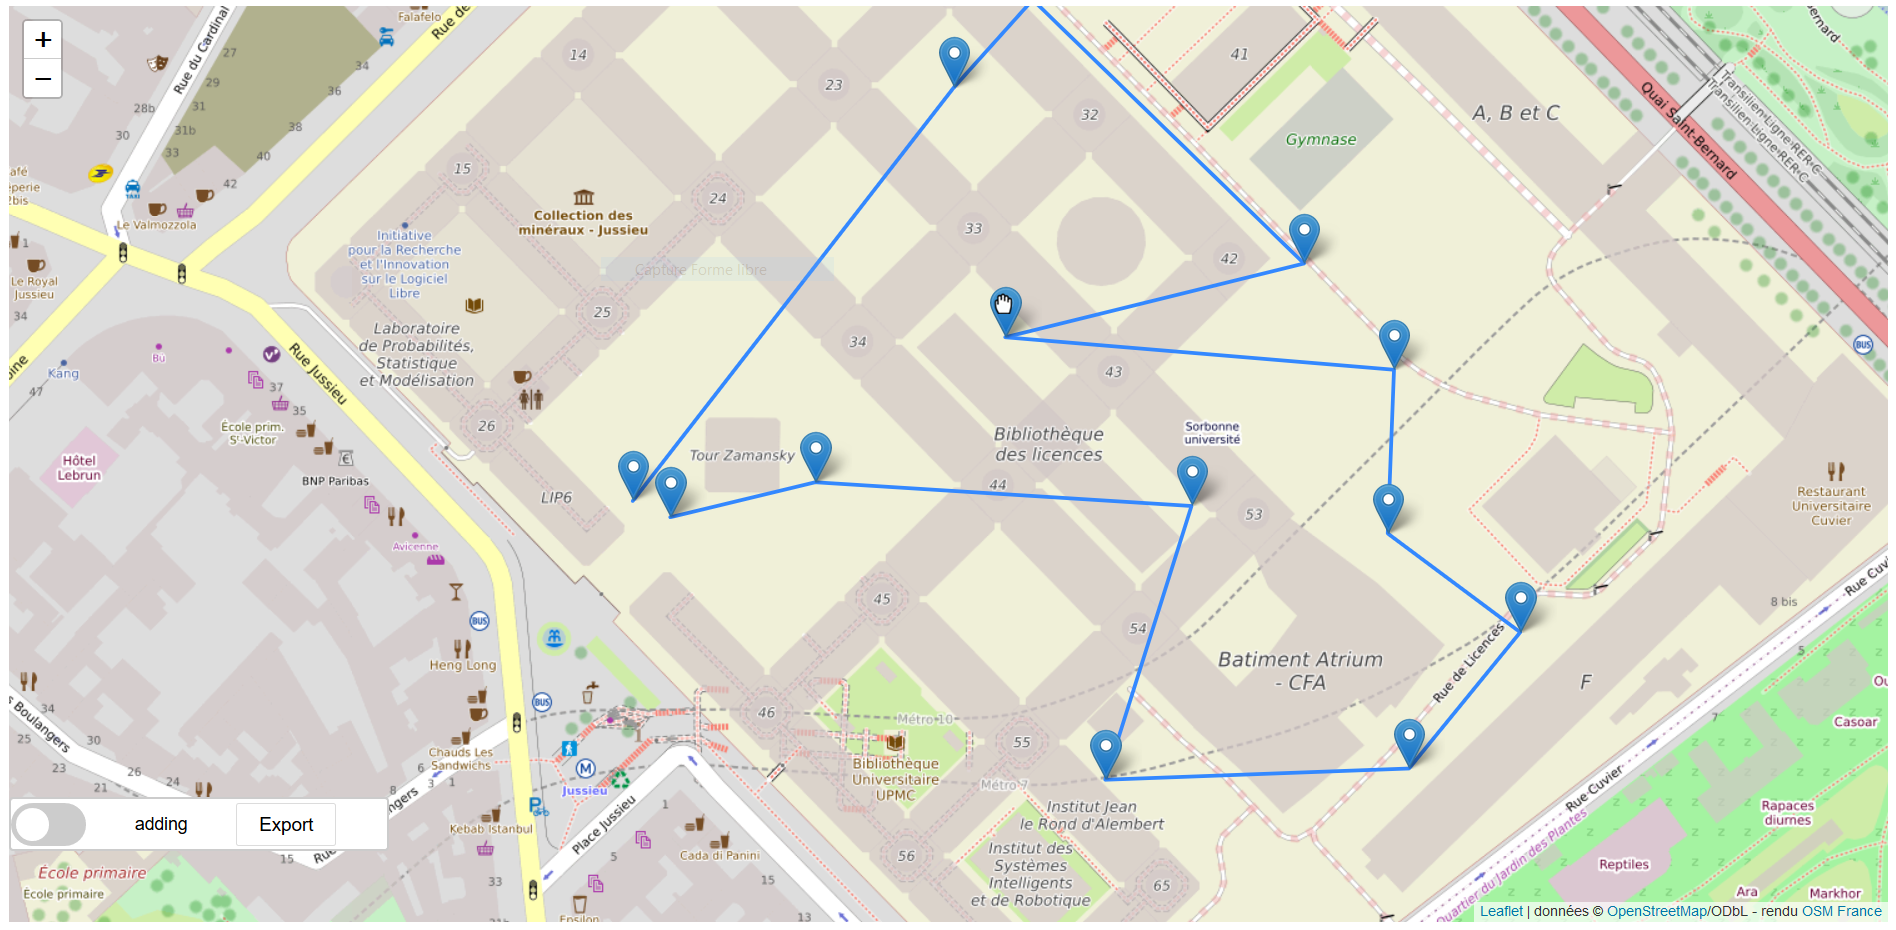
\includegraphics[scale=0.42]{capt7.png}
 	\caption{déplacer les marqueurs}
 	\end{center}
 	\end{figure}
 	%________________ 	
 	
  	%Une fois le plan de vol terminé, on clique sur le bouton pour obtenir le fichier correspondant au trajet défini :
  	\item Une fois le plan de vol terminé, on clique sur le bouton pour obtenir le fichier correspondant au trajet défini :\\
  	%________________
  	\begin{figure}[!h]
 	\begin{center}
 	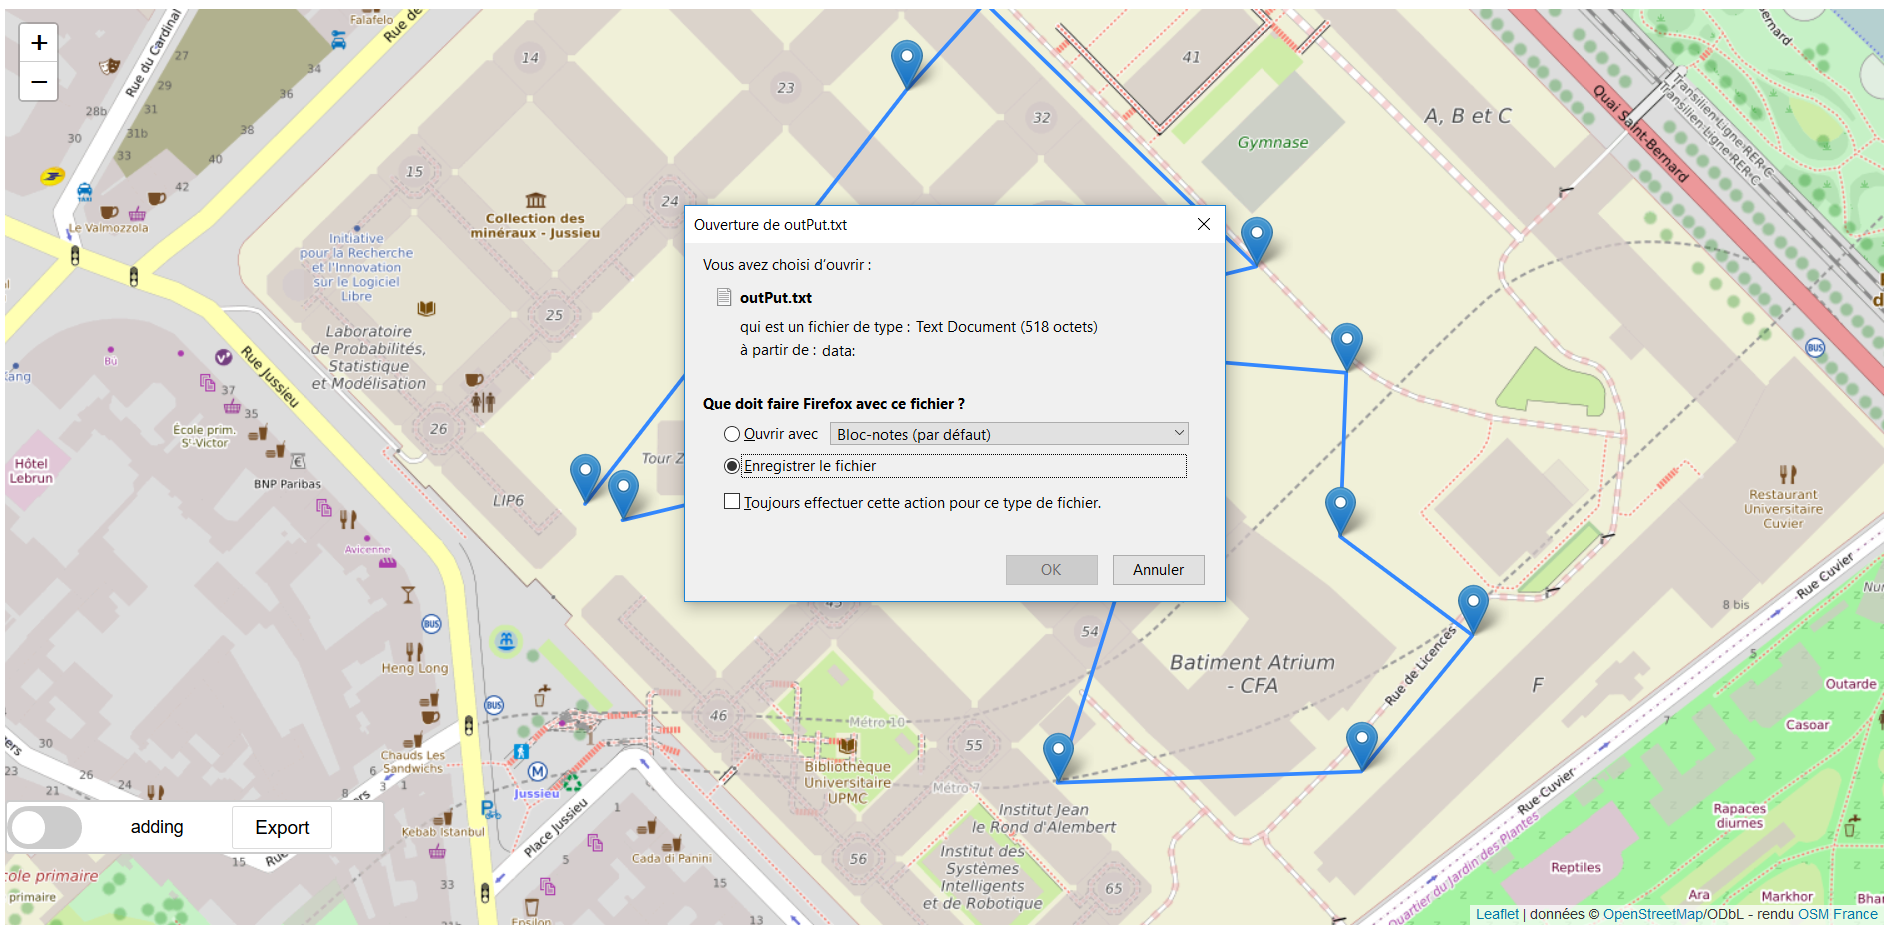
\includegraphics[scale=0.42]{capt8.PNG}
 	\caption{sauvegarde du plan}
 	\end{center}
 	\end{figure}
 	%________________ 	
 	\end{enumerate}
	\textit{Toutes ces images sont issues de prototypes d'interface graphique et sont non-contractuelles. Elles ne sont donc en aucun cas définitives et sont sujet à changement.}
	
% FIN CAHIER DES CHARGES %
    
        
	\newpage
\section{Architecture Logicielle}
    \subsection{Interface utilisateur}
    L'interface utilisateur est une interface GTK permettant d'intéragir avec le SDK Parrot afin d'enregistrer des trajets sur le drone et de les exécuter.
    \newline
    Elle permet également d'intéragir avec le Serveur local afin de saisir intéractivement le plan de vol à l'aide de l'application javascript et de créer les fichiers Mavlink.
    \vspace{0.2cm}
    \newline
    Voici l'architecture d'intéraction de l'interface utilisateur:
        \vspace*{0.5cm}
        \begin{center}
		\begin{figure}[!h]
		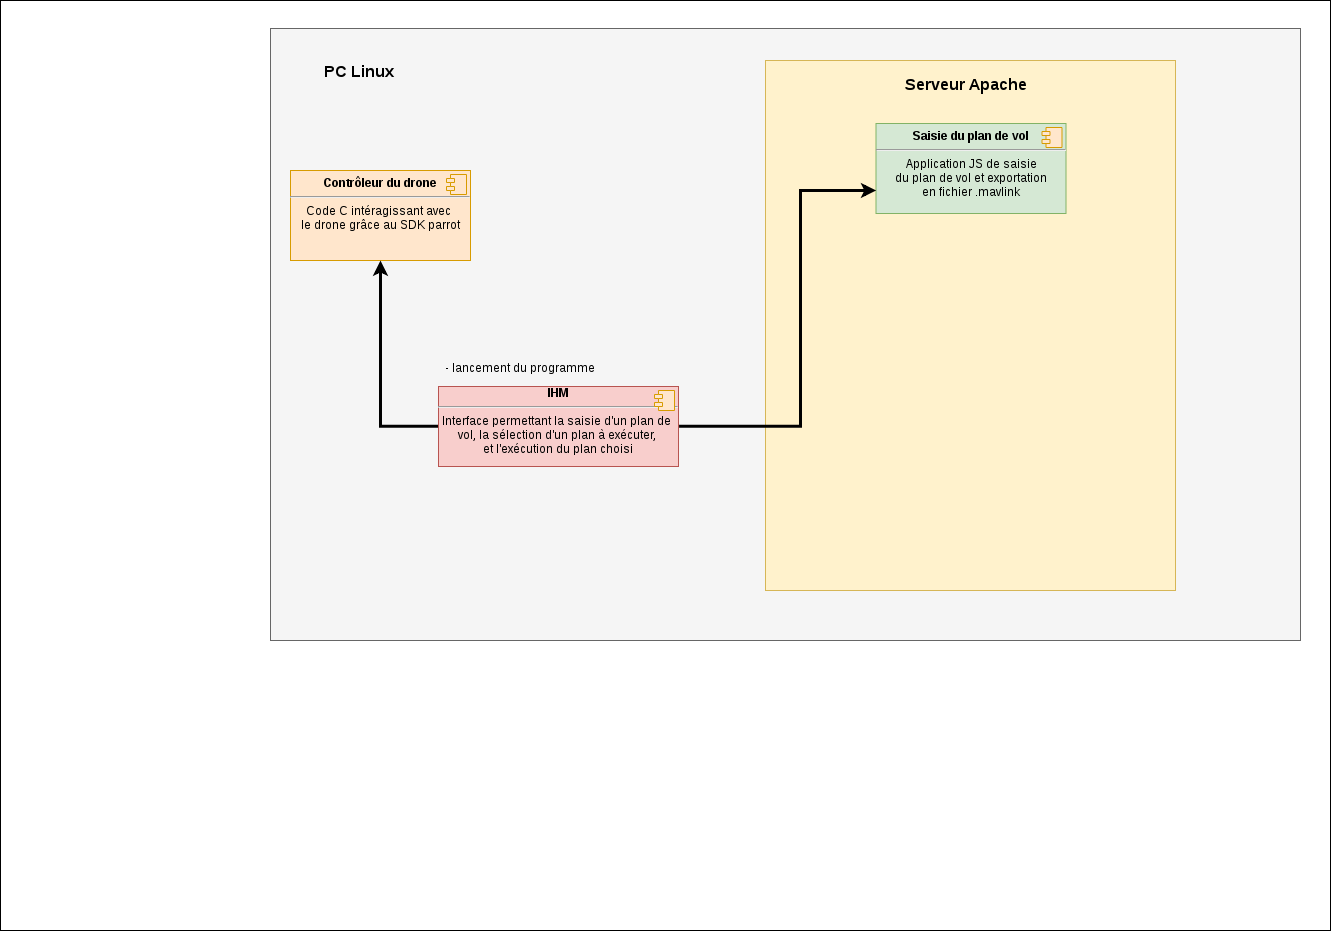
\includegraphics[scale=0.4]{01_archi_logicielle_IHM.png}\\
		 \vspace*{0.3cm}
		\caption{Interface utilisateur}
		\end{figure}
        \end{center}

\newpage
        
	 \subsection{Controle du drone}
	 Le contrôle du drone est axé autour de la génération du fichiers mavlink à l'aide de l'application JS sur le serveur local et du SDK Parrot qui permet d'envoyer des commandes au drone et de connaître son état.
	 \newline
	 Après avoir saisi interactivement un trajet à l'aide de l'application javascript, le fichier Mavlink généré et envoyé au SDK Parrot. 
	 \vspace{0.1cm}
	 \newline
	 
	 Le SDK permet ensuite le contrôle du drone à savoir:
	 \begin{enumerate}
        	\item Connexion au drone.
        	\item Exécution d'un plan de vol.
			\item Arrêt d'urgence.
    \end{enumerate}
    Le décollage et l'arrêt d'urgence du drone sont des commandes envoyées directement par le serveur, ses commandes seront envoyées au serveur par l'iPod afin de permettre un décollage et un arrêt ergonomique.
    \vspace{0.2cm}
    \newline
    Il permet également la réception de l'état du drone et du flux vidéo qui sera par la suite traité avec FFMPEG et envoyé en RTP à l'iPod.
    
	    \vspace*{0.3cm}
	    \begin{center}
		\begin{figure}[!h]
		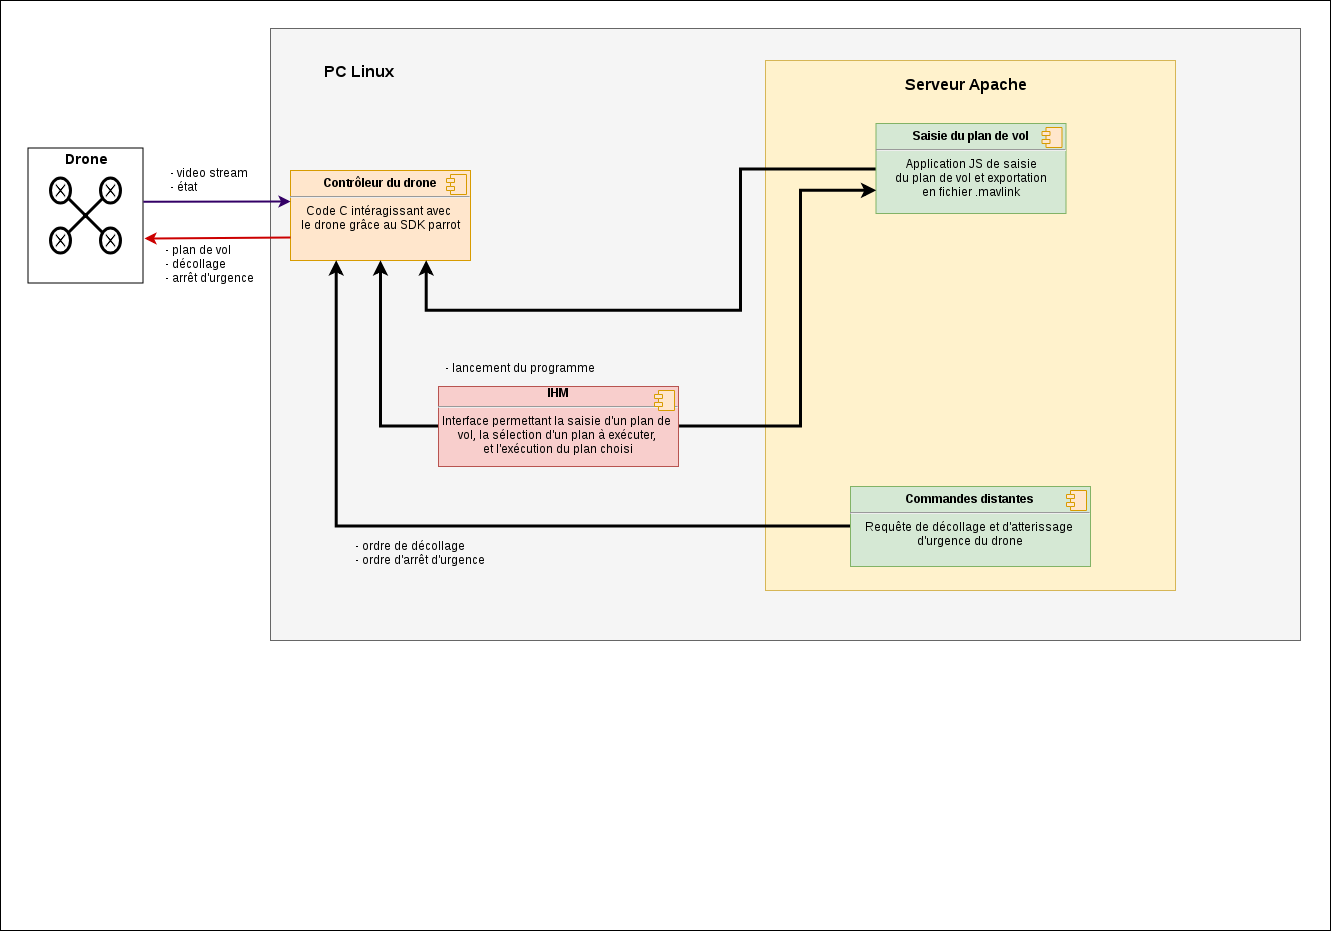
\includegraphics[scale=0.4]{02_archi_logicielle_controle_drone.png}\\
		\caption{Controle du drone}
		\end{figure}
        \end{center}
		
     \newpage
     \subsection{Application IOS}
     L'application IOS permet d'afficher le flux vidéo du drone et d'envoyer des requêtes au serveur en effectuant des gestes simples avec l'iPod afin de démarrage du drone et d'effectuer l'arrêt d'urgence.
     \vspace{0.2cm}
     \newline
     Dans un premier temps, l'application scanne le réseau afin de se connecter au serveur local.
     Après la connexion, une requête de demande de description du flux vidéo au format SDP est automatiquement envoyée au serveur.
     \vspace{0.2cm}
     \newline
     Le descripteur de flux est alors retourné par le serveur à l'application IOS, en parrallèle, elle reçoit également le flux video grâce au protocol RTP, le SDK VLC permet ensuite l'affichage vidéo.
        \vspace*{0.3cm}
	    \begin{center}
		\begin{figure}[!h]
		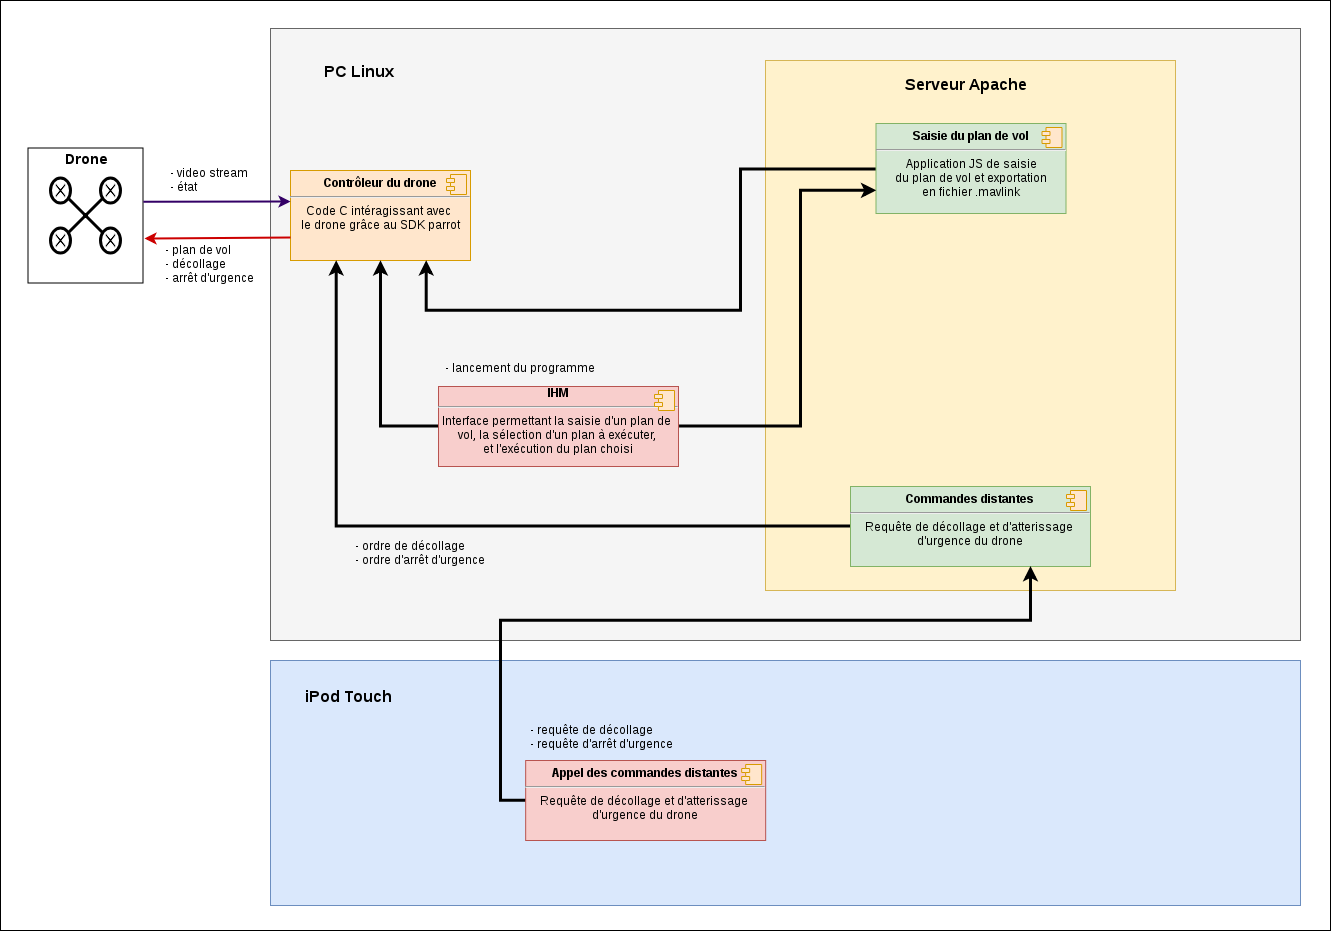
\includegraphics[scale=0.4]{03_archi_logicielle_iPod.png}\\
		\caption{Application IOS}
		\end{figure}
        \end{center}
        
    \newpage
	
	\subsection{Architecture logicielle globale}
	    \vspace*{0.3cm}
	    \begin{center}
		\begin{figure}[!h]
		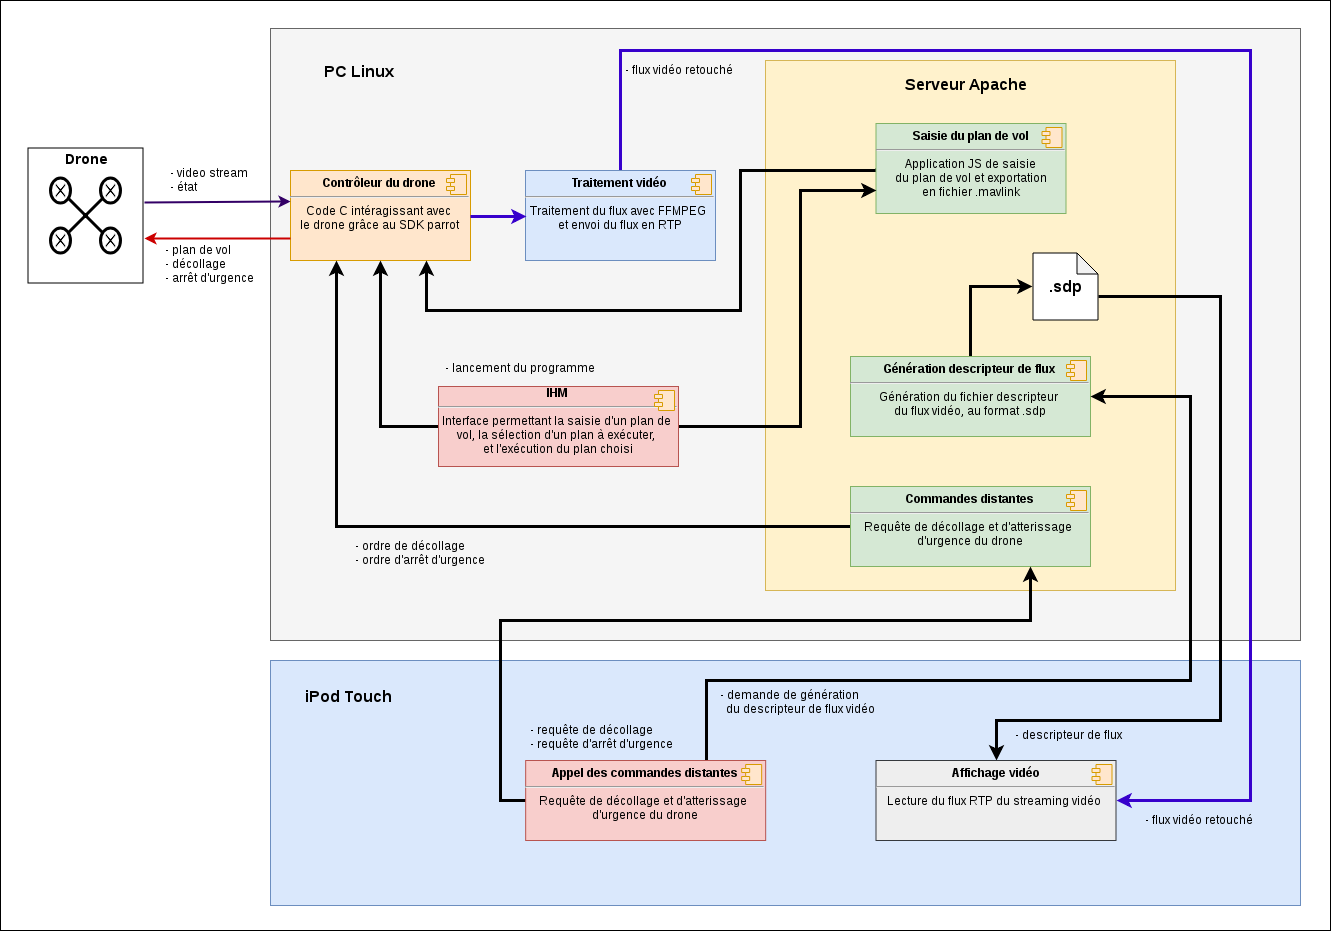
\includegraphics[scale=0.4]{04_archi_logicielle_complete.png}\\
		\caption{Architecture logicielle}
		\end{figure}
        \end{center}
		
\newpage
\section{Problèmes rencontrés}
	\subsection{Problèmes matériels}
	
	Nous avons rencontré plusieurs difficultés d'ordre matérielles lors de ce projet.
	\medbreak
	Tout d'abord nous avons été confrontés à un problème de GPS sur le campus de Sorbonne Université, en effet la couverture GPS était très mauvaise et les vols d'essai n'étaient donc possibles que très rarement. Nous avons eu l'occasion, avec l'accord de policiers en service présents sur les lieux, de faire des vols d'essai aux arènes de Lutèces à Jussieu. La couverture GPS y était très bonne et nous avons pu mener à bien nos tests. Malheureusement, nous n'avons pas eu d'autres occasions de faire voler le drone dans un environnement adapté et n'avons donc pas pu effectuer tous les tests voulus.
	\medbreak
	Ensuite, nous avons rencontré une difficulté lors du développement de l'application de l'iPod : nous avions besoin des composants VLC compatibles avec le logiciel de développement xCode, afin de faire fonctionner la récupération et l'affichage du flux vidéo par l'iPod. Nous ne disposions pas des droits nécessaires pour installer ces composants logiciels à la PPTI. Le logiciel de développement xCode ne fonctionnant que sur les appareils Apple, nous avons du nous procurer un ordinateur Mac et installer dessus les outils requis pour pouvoir continuer le projet.
	\medbreak
	Concernant le déploiement, nous avons du utiliser une machine virtuelle afin de procéder aux installations de test car nous ne disposions pas des droits nécessaires sur les machines de la PPTI.
	
	
\section{Organisation du travail}
	\subsection{Diagramme de Gantt}
    Les différentes étapes du projet sont visibles sur ce diagramme de Gantt, qui représente les tâches effectuées chaque semaine:
    \begin{center}
	\begin{figure}[!h]
	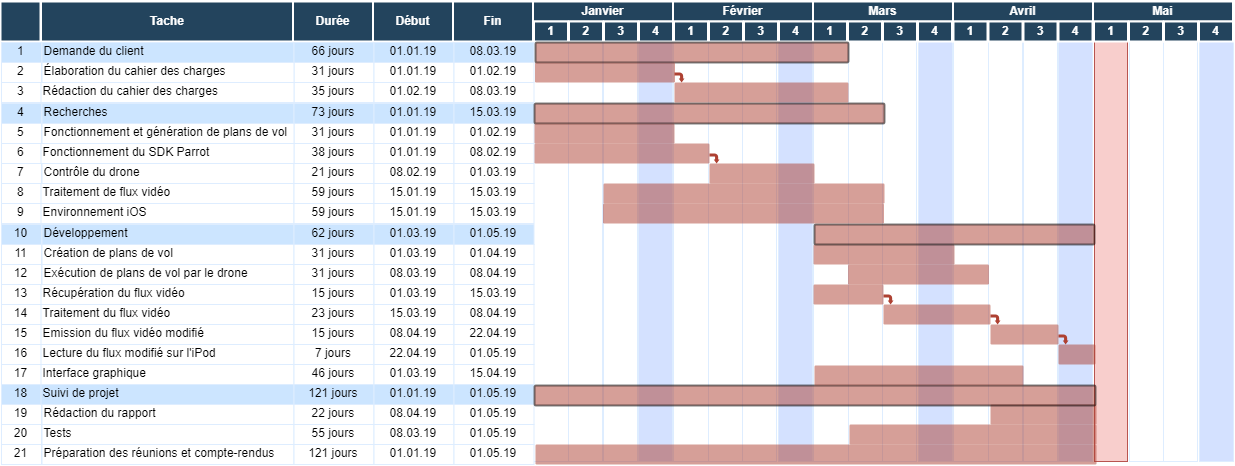
\includegraphics[scale=0.4]{gantt.png}
	\caption{Diagramme de Gantt du projet}
	\end{figure}
    \end{center}
    
    On y distingue les deux phases principales du projet : dans un premier temps la phase de recherche et de construction du cahier des charges, et dans un second temps la phase de développement et de mise en fonctionnement de l'application.
    
    \newpage
	\subsection{Répartition des taches}
	La répartition du travail durant ce projet est visible sur ce diagramme :
	
    \begin{center}
	\begin{figure}[!h]
	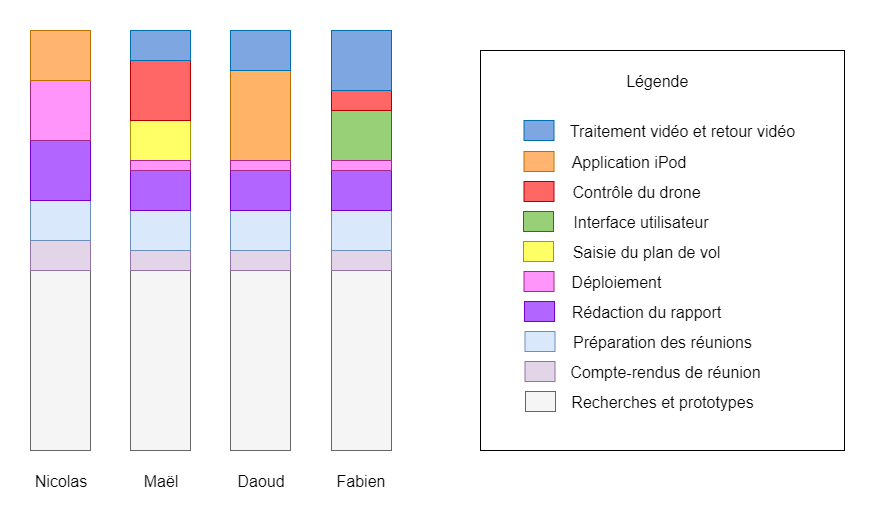
\includegraphics[scale=0.35]{repartition_taches.png}
	\caption{Répartition du travail}
	\end{figure}
    \end{center}
    
	Afin de ne pas avoir de retard sur les différentes taches à réaliser, nous avons réparti le travail équitablement entre les membres du groupe. Nous avons pu paralléliser les tâches majeures afin de bénéficier de tout le "man-power" disponible.\\
	
\section{Déploiement}

	Concernant le déploiement nous avons décidé de fournir une archive .zip au client avec deux scripts permettant l'installation et la désinstallation de l'application au travers d'un makefile. Le client n'utilisera pas directement les script mais interagira avec le makefile qui appellera les scripts bash. Nous n'avons pas pris en charge l'installation des composants annexes nécessaires à l'installation de l'application par manque de temps. Ces composants sont, par ordre d'importance, le serveur local lampp qui permet de gérer la partie création et sauvegarde des plan de vols (fichiers mavlink) ainsi que la redirection du flux vidéo provenant du drone et ayant pour destination l'iPod touch. L'installation et la configuration d'un serveur local lampp n'est pas compliqué mais demande beaucoup de temps. Il existe beaucoup de tutoriels sur le net pour installer un serveur lampp. Le second composant le plus important et FFmpeg. Ce logiciel permet de décoder, traiter, encoder et diffuser un flux vidéo. Il s'installe facilement avec un simple 'apt-get install ffmpeg'. Le dernier composant essentiel pour le client est la bibliothèque graphique GTK3.0 (ou version suppérieur). Notre application peut très bien tourner sans aucune interface graphique mais c'est beaucoup moins pratique. L'installation de cette bibliothèque peut être très compliqué si le client ne possède pas ubuntu 18.04 ou une version supérieur (GTK3 est préinstallé sur cette distribution).\\

Principe de fonctionnement de notre solution de déploiement :
Le client interagit avec un makefile qui affiche une page d'aide comme règle par défaut et lance deux scripts 'install.sh' et 'uninstall.sh'. Pour lancer l'installation le client saisira dans un terminal ouvert dans le répertoire de l'application 'make install' et pour supprimer l'application 'make uninstall'.\\
L'application est séparée en 3 archives à savoir la partie serveur, la partie contrôleur de drone et la partie interface graphique. La première action du script d'installation et de s'assurer que l'application n'est pas déjà installée sur le PC du client. Si elle l'est on laisse le choix au client de réinstaller ou de garder la version déjà installée.\\
Ces archives sont ensuite copiées et décompressées dans les bons répertoires par le script d'installation. Ces répertoires sont /var/www/public pour l'archive serveur, /usr/Bebop2App pour le contrôleur de drone et l'interface graphique.
Enfin le script termine par ajouter à la variable PATH du client le chemin d'accès vers le dossier contenant le main() principal de l'Application.\\

Le script de désinstallation supprime l'application et tous ces composants en parcourant les différents répertoires où les archives on été précédemment copiées et décompressées par le script d'installation. Après désinstallation il ne reste aucun fichier de l'application.\\

	\begin{center}
	\begin{figure}[!h]
	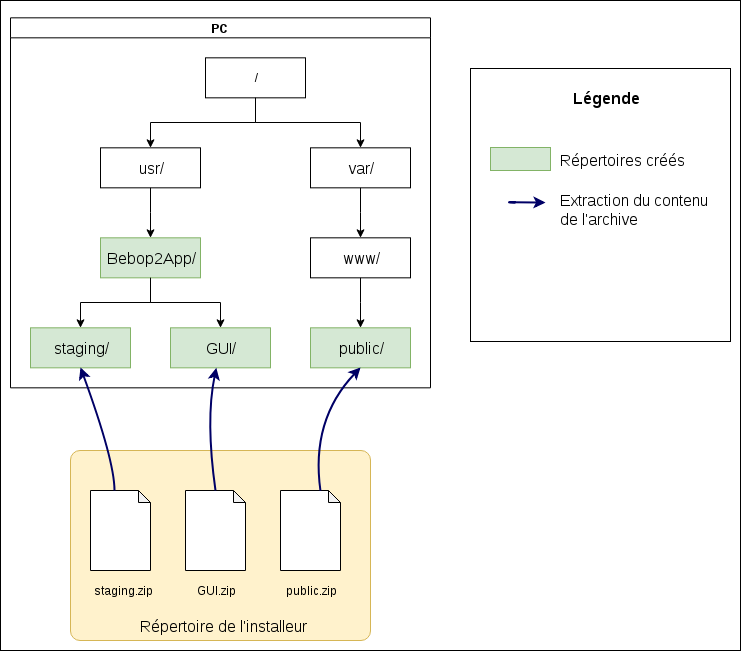
\includegraphics[scale=0.4]{deploiement.png}
	\caption{Schéma d'organisation du déploiement de l'application}
	\end{figure}
    \end{center}
    
    
\newpage
\section{Comparatif aux objectifs fixés}

\begin{center}
	    \vspace*{0.7cm}
        \begin{tabularx}{15cm}{|c|p{3cm}|p{5cm}||X|}
            \hline
            N° & Titre de l'objectif & détail (cahier des charges) & réalisation de l'objectif\\
            \hline
            1 & Saisie du plan de vol & L'utilisateur doit pouvoir saisir un plan de vol sur une carte à travers une interface intuitive. L'utilisateur doit pouvoir spécifier l'altitude du drone à chaque waypoint (point de passage).& L'utilisateur peut saisir un plan de vol sur une carte, et peut spécifier l'altitude pour chaque waypoint.\\
            \hline
            2 & Traduction du plan de vol au format Mavlink & Le plan de vol saisi graphiquement par l'utilisateur doit être converti au format Mavlink pour être ensuite envoyé au drone.& Le plan de vol est exporté au format Mavlink et stocké sur le serveur avec un nom choisi par l'utilisateur.\\
            \hline
            3 & Envoi du plan de vol au drone & La solution doit prendre en charge la récupération du plan de vol réalisé au préalable et son envoi au drone. & Le plan de vol choisi dans la fonctionnalité d'exécution de plan de vol est automatiquement transféré au drone.\\
            \hline
            4 & Choix du plan de vol  & L'utilisateur doit pouvoir choisir le plan de vol enregistré sur le drone qu'il souhaite exécuter. & L'utilisateur choisit dans un navigateur de fichier le plan de vol qu'il souhaite exécuter. Les plans de vol sont stockés sur le serveur, et seul le plan de vol choisi est envoyé au drone (pour ne pas surcharger la mémoire du drone). \\
            \hline
            5 & Exécution du plan de vol  & Une fois le plan de vol choisi, l'utilisateur doit pouvoir en lancer l'exécution. & Le bouton d'exécution du plan de vol permet de choisir le plan de vol et en lance l'exécution.\\
            \hline
            6 & Retour vidéo  & Tout au long du vol du drone, le retour vidéo de ce dernier doit être envoyé sur un iPod touch en temps réel et avec une latence minimale. & Une fois l'application iPod lancée et l'exécution du plan de vol demandée, la vidéo prise par le drone en temps réel est transférée à l'iPod avec une vue FPV (une image pour chaque oeil), avec une latence d'environ 6 secondes. La qualité d'image est celle fournie par le drone : résolution 480x856px. \\
            \hline
            7 & Arrêt d'urgence  & À tout moment un deuxième utilisateur doit pouvoir enclencher un arrêt d'urgence depuis le PC. & Pour des raisons pratiques et après discussion avec le client, cette fonctionnalité est remplacée par l'arrêt d'urgence par un mouvement de tête.\\
            \hline
            8 & Démarrage de la ronde à l'aide de gestes & L'utilisateur pourra éventuellement engager le démarrage du vol en effectuant un certain mouvement de la tête. & Une fois l'exécution du plan de vol lancé, le drone attend l'autorisation de décoler qui est donnée par un hochement de tête avec l'iPod Touch.	\\
			\hline
			9 & Arrêt d'urgence & L'utilisateur pourra éventuellement engager un arrêt d'urgence en effectuant par exemple un certain mouvement de la tête. & Une fois le drone en vol, l'arrêt d'urgence peut être activé par un hochement de tête avec l'iPod Touch.	\\
			\hline
        \end{tabularx}
        \end{center}
	
\newpage
\section{Améliorations possibles}
Tout d'abord, une amélioration de l'application de saisie du plan de vol serait possible afin de permettre à l'utilisateur de choisir dans quelle direction le drone doit regarder au fur-et-à-mesure du vol.
\medbreak
Ensuite, l'application utilisée pour la lecture de la vidéo est conçue pour un iPod Touch. Compte tenu de la nature universelle du protocole utilisé pour envoyer le flux vidéo (protocole RTP), il est tout à fait possible de développer des applications similaires compatibles à d'autres systèmes. Il est d'ailleurs d'ores et déjà possible de lire la vidéo depuis un appareil androide à l'aide de la fonctionnalité de lecture de flux de l'application VLC, ce qui est plus contraingant à paramétrer que s'il existait une application dédiée bien évidemment.
\medbreak
Concernant la latence du retour vidéo qui est d'environ 6 secondes sur les appareils que nous avons utilisés, nous pensons qu'il est possible de diminuer ce délai en utilisant une connexion wifi directe entre l'iPod et le PC linux, plutôt que de passer par un réseau local servant d'intermédiaire.

\section{Conclusion}

Nous avons mis en œuvre une solution utilisant le PC Linux ainsi que l'iPod Touch afin de répondre aux besoins du client, et nous avons rencontré des obstacles auxquels nous n'avons malheureusement pas pu trouver de solutions pour certains.\\
En effet, en ce qui concerne le déploiement, celui-ci n'est pas automatique dans son intégralité, et permet simplement l'installation des fichiers sources que nous avons réalisés. Les utilitaires comme FFMPEG, le serveur LAMP ou la bibliothèque GTK ne seront pas installées par le biais de notre déploiement, mais devront être préalablement configurés sur la machine du client.\\
La couverture GPS étant très mauvaise à Jussieu, nous n'avons pas eu l'occasion d'effectuer nos tests de vols dans de bonne conditions.\\
Effectivement, le changement d'angle de la caméra du drone (yaw) lorsque celui-ci tourne n'était pas fonctionnel à tous les essais, et nous soupçonnons la mauvaise couverture GPS d'être à l'origine de cette erreur.\\
Malgré ces inconvenues, le projet est un succès sur de nombreux points.\\
En effet, l'interface utilisateur permet de saisir de façon simple des plan de vol utilisables par le drone, et ils peuvent être gérés et sélectionnés par l'utilisateur de manière intuitive. Le plan de vol choisi est ensuite transmis au drone.\\
La vidéo de la caméra du drone est correctement retransmise à l'iPod Touch en temps réel, et est adaptée au visionnage dans un masque FPV grâce à un dédoublement de l'image. La latence du retour vidéo est d'environ 6 secondes, ce qui est convenable dans ce contexte d'utilisation.\\
D'un point de vue ergonomique, le démarrage de la ronde ainsi que l'arrêt d'urgence du drone s'effectuent grâce à un mouvement de la tête, ce qui permet à l'utilisateur de garder le masque FPV durant tout le vol sans avoir à effectuer de manipulation complexe.

	
 
\end{document}
